\documentclass[12pt]{article}

%%%%%%%%%%%%%%%%%%%%%%%%%%%%%%%%%%%%%%%%%%%%%%%%%%%%%
% ARQUIVOS RELACIONADOS INCLUIDOS

% pacotes customizados
\input{resources/packages.tex}

% comandos customizados
\input{resources/custom_commands.tex}

%%%%%%%%%%%%%%%%%%%%%%%%%%%%%%%%%%%%%%%%%%%%%%%%%%%%%
% PARAMETROS DO DOCUMENTO

% titulo do documento
\titulo{Trabalho de Informática Industrial}

% subtitulo do documento
% 	*Veja que o simbolo '~' não é renderizado, se tratando de um 'placeholder'.
\subtitulo{Dry-Martini}

% adicione a descricao do trabalho que aparece na contra-capa
\descricao{Sistema de Automação de Produção de Dry Martini}

% nome dos autores. Separe-os por '\\'
\autores{Rian Rero Lopes Jericó Vieira \\ Lara Strutz Carvalho \\ Luis Otávio de Souza Silva}
	
% departamento
\departamento{Departamento de Engenharia Eletrônica}	

% professor
\professor{Prof. Emerson Alves da Silva}

% codigo da disciplina
\disciplina{ELT008}

% turma
\turma{TECAN}
	
% data do documento
\data{\today}	


%%%%%%%%%%%%%%%%%%%%%%%%%%%%%%%%%%%%%%%%%%%%%%%%%%%%%
% INICIO DO DOCUMENTO
\begin{document}
\begin{titlepage}

\input{resources/front_page.tex}

%%%%%%%%%%%%%%%%%%%%%%%%%%%%%%%%%%%%%%%%%%%%%%%%%%%%%
%%%%%%%%%%%%%%%%%%%%%%%%%%%%%%%%%%%%%%%%%%%%%%%%%%%%%
% *COLOQUE SUAS SEÇÕES TEXTUAIS AQUI
\section{Introdução}\label{sec:introducao}

Este relatório tem como objetivo documentar o desenvolvimento de uma aplicação de supervisão e controle utilizando o software \textbf{CODESYS v3.5}\cite{codesysV35SP21} e o supervisório \textbf{InduSoft Web Studio}. O projeto contempla a automação de uma planta de produção de Dry Martini, abrangendo desde a dosagem e mistura dos ingredientes (Área 01) até o envase e transporte do produto final (Área 02).

O sistema desenvolvido integra lógicas sequenciais (SFC), controle contínuo (Ladder), algoritmos matemáticos (Texto Estruturado) e comunicação via protocolo \textbf{OPC UA}. A aplicação foi estruturada em tarefas multitarefa para garantir a fidelidade da simulação física e a precisão do controle.

Este documento detalha a divisão das tarefas, a lógica implementada em cada Unidade de Organização de Programa (POU) e a interface desenvolvida para operação.

Todo o projeto pode ser encontrado no Git-Hub atráves do url:  \url{https://github.com/Rian-Rero/Dry-Martini}\cite{dryMartiniRepo}
\section{Divisão de Tarefas e Programas da Aplicação}\label{sec:div-tarefas}

A arquitetura do software foi dividida em tarefas distintas para separar a lógica de controle da lógica de simulação física, garantindo determinismo e tempos de ciclo adequados e requisição de multi-task.

\subsection{MainTask (PrgBatelada)}
\begin{itemize}
    \item \textbf{Tempo de Ciclo:} 20 ms.
    \item \textbf{Prioridade:} 1.
    \item \textbf{Descrição:} Responsável pela execução da lógica de controle sequencial da batelada em SFC. Essa task controla o armazenamento e dosagem de matéria-prima. Esta seção é responsável pelo gerenciamento dos reservatórios iniciais. A lógica de controle desenvolvida atua sobre as válvulas de saída e bombas de transferência, garantindo que o volume exato requisitado pela receita seja transportado para o estágio seguinte. O controle nesta etapa é essencial para assegurar a proporção correta dos ingredientes antes do início do processamento da batelada. Além disso a lógica de emergência em que todos os procedimentos são pausados e o tanque da Área 01 esvaziado antes que o processo de produção seja reestabelecido. Contém o programa: \texttt{PrgBatelada}.
\end{itemize}

\subsection{T\_ENVASE (PrgArea02\_Envase)}
\begin{itemize}
    \item \textbf{Tempo de Ciclo:} 50 ms.
    \item \textbf{Prioridade:} 1.
    \item \textbf{Descrição:}
A Área 02 destina-se ao processo de envase do produto final, operando de forma integrada entre o Tanque de Produto (TP-01) e o Transportador (TR-01) para o enchimento de barris de 15 litros. O ciclo automatizado inicia-se quando o nível do TP-01 atinge 50\%, habilitando o motor da esteira (M-201), que é interrompido momentaneamente ao detectar a presença de um tonel via sensor ZY-201 para permitir a abertura da válvula de envase (FV-201). O controle volumétrico é realizado pelo totalizador FQ-201 que, ao atingir o setpoint de 15L, comanda o fechamento da válvula e a retomada do transporte, sendo os tonéis contabilizados posteriormente pelo sensor ZY-202. O sistema incorpora lógicas de intertravamento e segurança que monitoram os níveis críticos do TP-01 — gerando alarmes em níveis altos (85\% e 95\%) e bloqueando o envase caso o nível desça a 10\% (LSL-201), com histerese para religamento apenas em 50\% — além de supervisionar a alimentação da linha, interrompendo o processo e gerando alarme caso nenhum barril seja detectado num intervalo de 15 segundos.Contém o programa: \texttt{PrgArea02\_Envase}.
\end{itemize}
\subsection{T\_PRG (PLC\_PROG)}
\begin{itemize}
    \item \textbf{Tempo de Ciclo:} 20 ms.
    \item \textbf{Prioridade:} 1.
    \item \textbf{Descrição:}
    Esta task é responsável pelo gerenciamento das variáveis internas de controle. A lógica implementada processa a comutação (toggle) do botão de modo automático e atualiza a variável correspondente no CPL, habilitando a inicialização autônoma do processo. Simultaneamente, esta tarefa centraliza o monitoramento e o tratamento de todos os alarmes de nível do sistema.Contém o programa: \texttt{PLC\_PROG}.
\end{itemize}
\subsection{T\_PWM (PrgPWM\_M101)}
\begin{itemize}
    \item \textbf{Tempo de Ciclo:} 5ms.
    \item \textbf{Prioridade:} 1.
    \item \textbf{Descrição:}

Para atender aos requisitos de acionamento suave do motor M-101, implementou-se um algoritmo de Modulação por Largura de Pulso (PWM) operando na frequência de 20 Hz, estruturado para gerenciar rampas lineares de aceleração e desaceleração. A lógica utiliza o tempo decorrido (Elapsed Time - ET) de temporizadores específicos para calcular dinamicamente o ciclo de trabalho (duty\ cycle), promovendo uma variação de 0 a 100\% em 5 segundos durante a partida e de 100 a 0\% em 10 segundos no desligamento. A geração do sinal de saída para o relé de estado sólido (GVL.xSY101\_PWM\_Out) é realizada através da comparação contínua entre um temporizador cíclico de base (tCycleTimer) e a largura de pulso proporcional à velocidade calculada, assegurando a modulação correta da tensão média aplicada ao atuador \texttt{SY-101} dentro dos limites de segurança estabelecidos.
\end{itemize}



\subsection{T\_SIMULACAO (PrgSimulacao)}
\begin{itemize}
    \item \textbf{Tempo de Ciclo:} 100ms.
    \item \textbf{Prioridade:} 1.
    \item \textbf{Descrição:}
Para a validação da lógica de controle sem a presença da planta física, utilizou-se a estratégia de simulação baseada nos blocos funcionais (FBs) RMISTURA e TPRODUTO, fornecidos especificamente para emular a dinâmica do Reator de Mistura e do Tanque de Produto. Estes blocos foram instanciados em linguagem Ladder e configurados para responder aos acionamentos das válvulas e motores, gerando os sinais de nível e sensores discretos correspondentes. Um aspecto crítico desta etapa foi o ajuste do tempo de ciclo da tarefa (Task) no ambiente multitarefa do CODESYS, visto que as vazões simuladas são dependentes dessa discretização temporal. A integridade da simulação foi verificada através da ferramenta de monitoramento gráfico (Trace), assegurando que os tempos de enchimento e esvaziamento dos tanques correspondessem às vazões de projeto estipuladas.Contém o programa: \texttt{PrgSimulacao}.
\end{itemize}
\section{Relação de Variáveis}\label{sec:var-relations}

As variáveis globais do sistema estão categorizadas por sua função no processo de automação.

\subsection{Entradas e Sensores (Instrumentação)}


\begin{description}
    \item[\texttt{LSH101} / \texttt{LSL101}] Sensores digitais de nível Alto e Baixo do Reator de Mistura (RM-01).
    \item[\texttt{LSH102} / \texttt{LSL102}] Sensores digitais de nível Alto e Baixo da Jaqueta de Resfriamento.
    \item[\texttt{TSL101}] Termostato digital que indica se a temperatura de processo foi atingida (Temperatura OK).
    \item[\texttt{LSHH201}] Sensor de nível ``Muito Alto'' (segurança) do Tanque de Produto (TP-01).
    \item[\texttt{LSH201} / \texttt{LSL201}] Sensores digitais de nível Alto e Baixo do Tanque de Produto (TP-01).
    \item[\texttt{ZY201\_Detect}] Sensor óptico para detecção de presença de barril na posição de envase.
    \item[\texttt{ZY202\_Conta}] Sensor de saída da esteira responsável pela contagem de barris finalizados.
    \item[\texttt{rNivel\_RM01} / \texttt{rNivel\_TP01}] Variáveis analógicas (LREAL) que recebem a leitura dos transmissores de nível dos tanques.
    \item[\texttt{rVelocidade\_Misturador}] Feedback (retorno) da velocidade real do motor do misturador.
    \item[\texttt{rVolume\_RM01} / \texttt{rVolume\_TP01}] Variáveis calculadas que representam o volume atual dentro dos respectivos tanques.
\end{description}

\subsection{Saídas e Atuadores}
Variáveis responsáveis pelo comando físico dos equipamentos de campo.

\begin{description}
    \item[\texttt{FV101} / \texttt{FV102}] Válvulas solenoides de entrada de matéria-prima (Gin e Vermouth) no Reator.
    \item[\texttt{FV103}] Válvula de entrada de líquido refrigerante na Jaqueta.
    \item[\texttt{FV104}] Válvula de descarga do Reator para transferência de produto.
    \item[\texttt{FV105}] Válvula de admissão do Tanque de Produto.
    \item[\texttt{FV106} / \texttt{FV107}] Válvulas de dreno/rejeitos do Reator e da Jaqueta, respectivamente.
    \item[\texttt{FV201}] Válvula de envase (dosagem do produto no barril).
    \item[\texttt{BA101}] Comando da Bomba de Transferência.
    \item[\texttt{bM101\_Ligar}] Comando lógico para habilitar o motor do misturador.
    \item[\texttt{xSY101\_PWM\_Out}] Saída modulada (PWM) para controle de velocidade do inversor do misturador.
    \item[\texttt{bM201\_Esteira}] Comando de acionamento do motor da esteira transportadora.
\end{description}

\subsection{Comandos e Interface (HMI)}
Variáveis de interação com o operador e diagnósticos do sistema.

\begin{description}
    \item[\texttt{bBotaoAuto} / \texttt{bBotaoMan}] Botões de pulso para seleção do modo de operação (Automático ou Manual).
    \item[\texttt{bBotaoEmg}] Botão de Emergência (Geralmente NF) para paradas críticas.
    \item[\texttt{bResetAlarm}] Botão para reconhecimento e limpeza de alarmes ativos.
    \item[\texttt{bModoAutomatico}] \textit{Flag} interna de estado: \texttt{TRUE} indica operação automática ativa.
    \item[\texttt{bResetContador}] Comando para zerar os totalizadores de produção.
    \item[\texttt{iContadorBatelada} / \texttt{iContadorBarris}] Contadores de bateladas produzidas e barris envasados.
    \item[\texttt{rTotal\_Gin} / \texttt{rTotal\_Vermouth}] Totalizadores de volume consumido de matéria-prima.
    \item[\texttt{bAlarme\_...}] Conjunto de \textit{flags} que indicam falhas críticas (ex: Nível Alto, Transporte Vazio).
\end{description}
\section{Programas}\label{sec:programs}

\subsection{Controle da Batelada (PrgBatelada) - SFC}
Este programa implementa a receita de produção utilizando a linguagem \textbf{SFC (Sequential Function Chart)}, ideal para processos em etapas.

A sequência principal consiste em:
\begin{enumerate}
    \item \textbf{Init:} Verifica condições iniciais (Modo Automático, Sem Emergência, TP-01 não cheio).
    \item \textbf{Dosagem:} Abre \texttt{FV101} (Gin) e \texttt{FV102} (Vermouth) sequencialmente até atingir o volume alvo (45L).
    \item \textbf{Mistura e Resfriamento:} Liga o motor \texttt{M101} e abre a refrigeração \texttt{FV103}. Aguarda o nível da jaqueta e a temperatura (TSL101).
    \item \textbf{Transferência:} Drena a jaqueta (\texttt{FV107}) e transfere o produto (\texttt{BA101}, \texttt{FV104}, \texttt{FV105}) para o tanque pulmão.
    \item \textbf{Totalização:} Incrementa os totalizadores globais ao fim do ciclo.
\end{enumerate}

\subsubsection{Rotina de Emergência}
Foi implementada uma "Ilha de Emergência" no SFC. Em caso de acionamento do botão \texttt{EMG} em qualquer etapa crítica, o fluxo é desviado (via \textit{Alternative Branch}) para uma sequência de segurança que:
\begin{itemize}
    \item Fecha todas as admissões imediatamente.
    \item Aguarda 3 segundos.
    \item Configura válvulas de descarte para o Tanque de Rejeitos (\texttt{FV106}).
    \item Esvazia o reator com segurança antes de permitir o rearme.
\end{itemize}

\begin{figure}[H]
    \centering
    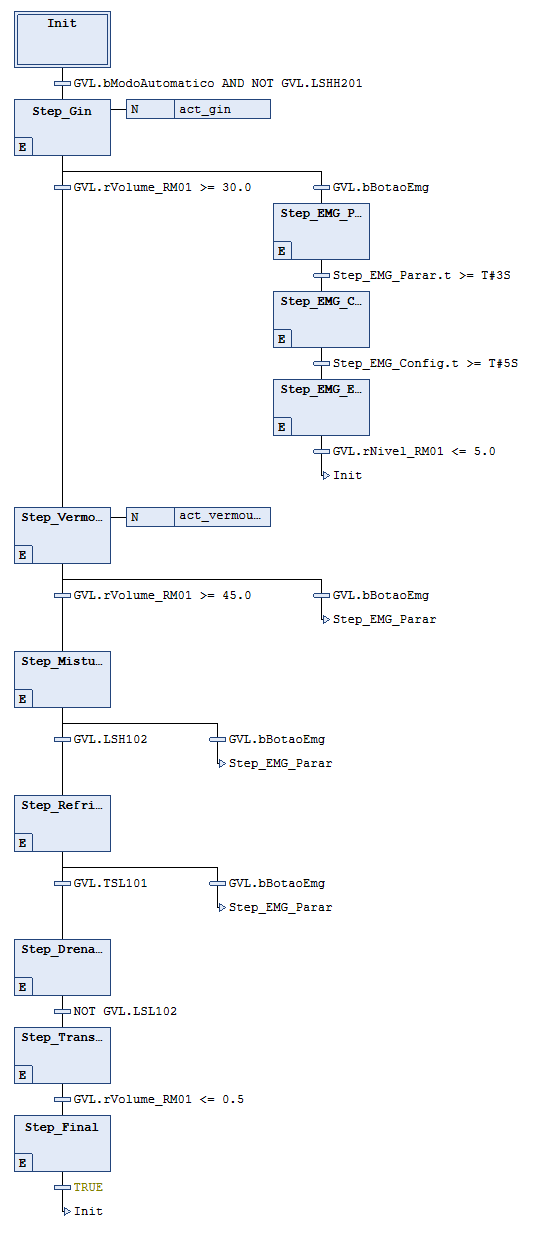
\includegraphics[width=0.6\textwidth]{imgs/SFC-Batelada.png} 
    \caption{Lógica SFC da Batelada com tratamento de Emergência.}
\end{figure}

\subsection{Controle PWM (PrgPWM\_M101) - Texto Estruturado}
Para atender ao requisito de controle de velocidade do misturador com rampas suaves, utilizou-se a linguagem \textbf{ST}.

\textbf{Lógica Implementada:}
\begin{itemize}
    \item \textbf{Rampas:} Dois temporizadores \texttt{TON} controlam a aceleração (0 a 100\% em 5s) e a desaceleração (100 a 0\% em 10s). O cálculo do \textit{Duty Cycle} é feito matematicamente a cada ciclo.
    \item \textbf{Geração de Pulso:} Um timer cíclico de 5ms gera a base de tempo para a frequência de 20Hz. A saída \texttt{xSY101\_PWM\_Out} permanece em nível alto proporcionalmente ao valor da rampa calculado.
\end{itemize}

\begin{lstlisting}
// --- 1. Controle dos Temporizadores ---
// Timer de Subida (5s)
tStartTimer(IN := GVL.bM101_Ligar AND NOT tStopTimer.Q, PT := T#5S);

// Timer de Descida (10s)
tStopTimer(IN := NOT GVL.bM101_Ligar AND NOT tStartTimer.Q, PT := T#10S);

//  2. Calculo da Rampa (0 a 100\%) 
IF tStartTimer.IN OR tStartTimer.Q THEN
    // Converte o tempo decorrido (ET) para Real para fazer a conta
    GVL.rVelocidade_Misturador := (TIME_TO_REAL(tStartTimer.ET) * 100.0) / 5000.0;

ELSIF tStopTimer.IN OR tStopTimer.Q THEN
    // Rampa de descida
    GVL.rVelocidade_Misturador := 100.0 - ((TIME_TO_REAL(tStopTimer.ET) * 100.0) / 10000.0);

ELSIF GVL.bM101_Ligar THEN
    GVL.rVelocidade_Misturador := 100.0;
ELSE
    GVL.rVelocidade_Misturador := 0.0;
END_IF

// Trava de seguranca (Limites)
GVL.rVelocidade_Misturador := LIMIT(0.0, GVL.rVelocidade_Misturador, 100.0);

// --- 3. Geracao do Pulso PWM (20 Hz) ---
tCycleTimer(IN := NOT tCycleTimer.Q, PT := tPeriodo);
IF tCycleTimer.Q THEN
    tCycleTimer(IN := FALSE);
END_IF

// Convertemos tudo para REAL (milissegundos) antes de comparar
GVL.xSY101_PWM_Out := TIME_TO_REAL(tCycleTimer.ET) < (TIME_TO_REAL(tPeriodo) * (GVL.rVelocidade_Misturador / 100.0));
\end{lstlisting}

\subsection{Controle de Envase (PrgArea02\_Envase) - Ladder}
A Área 02 foi desenvolvida em \textbf{Ladder Diagram (LD)} para controle de intertravamentos e lógica contínua.

\textbf{Funcionalidades Principais:}
\begin{itemize}
    \item \textbf{Histerese da Esteira:} A esteira liga apenas se o nível do TP-01 for superior a 50\% e desliga se for inferior a 10\% (utilizando lógica de Set/Reset e comparadores \texttt{GE} e \texttt{LT}).
    \item \textbf{Simulação de Enchimento:} Um bloco \texttt{ADD} incrementa o volume simulado do barril enquanto a válvula \texttt{FV201} está aberta.
    \item \textbf{Contagem:} Um contador \texttt{CTU} registra o número de barris produzidos (\texttt{iContadorBarris}) do tipo WORD.
\end{itemize}

\begin{figure}[H]
    \centering
    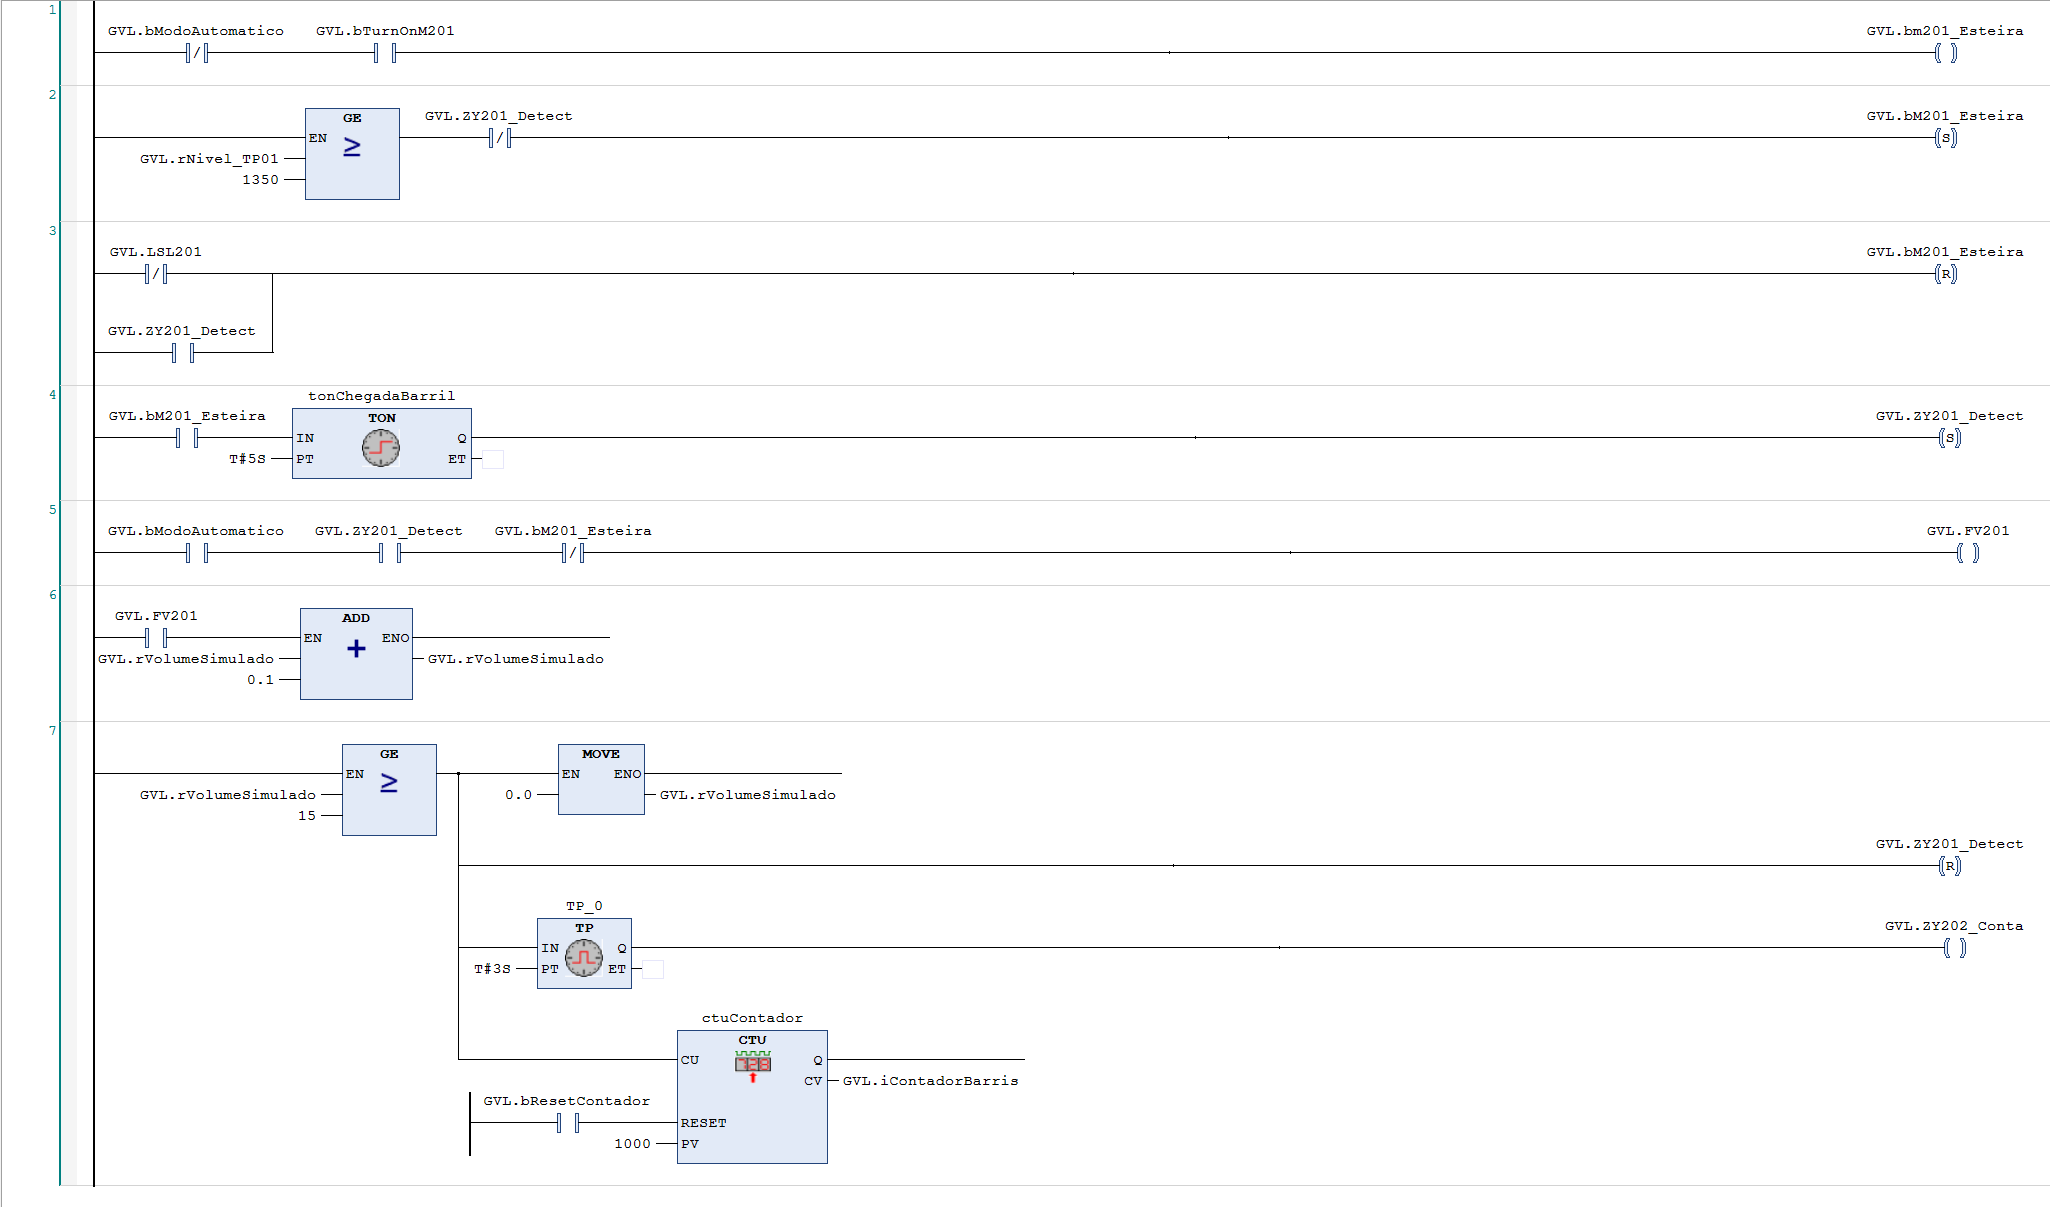
\includegraphics[width=1\textwidth]{imgs/Ladder-Envase.png}
    \caption{Lógica Ladder do controle de envase e esteira.}
\end{figure}

\subsection{Alarmes e Supervisão (PLC\_PRG) - Ladder}
Este programa centraliza a geração de alarmes e a lógica de conversão de sinais analógicos para discretos. Além disso, esse programa é responsável por mudar a variável interna de modo automático, quando o chave de seleção é alterada.
\begin{itemize}
    \item \textbf{Alarmes de Nível:} Comparadores monitoram \texttt{rNivel\_TP01} e acionam flags de alarme para Nível Baixo ($> 10\%$), Alto ($> 85\%$) e Muito Alto ($> 95\%$).
    \item \textbf{Alarme de Transporte:} Um temporizador \texttt{TON} de 15s dispara um alarme se a esteira estiver ligada sem detecção de barris, indicando falha de alimentação.
\end{itemize}


\begin{figure}[H]\label{fig:ladder-prg}
    \centering
    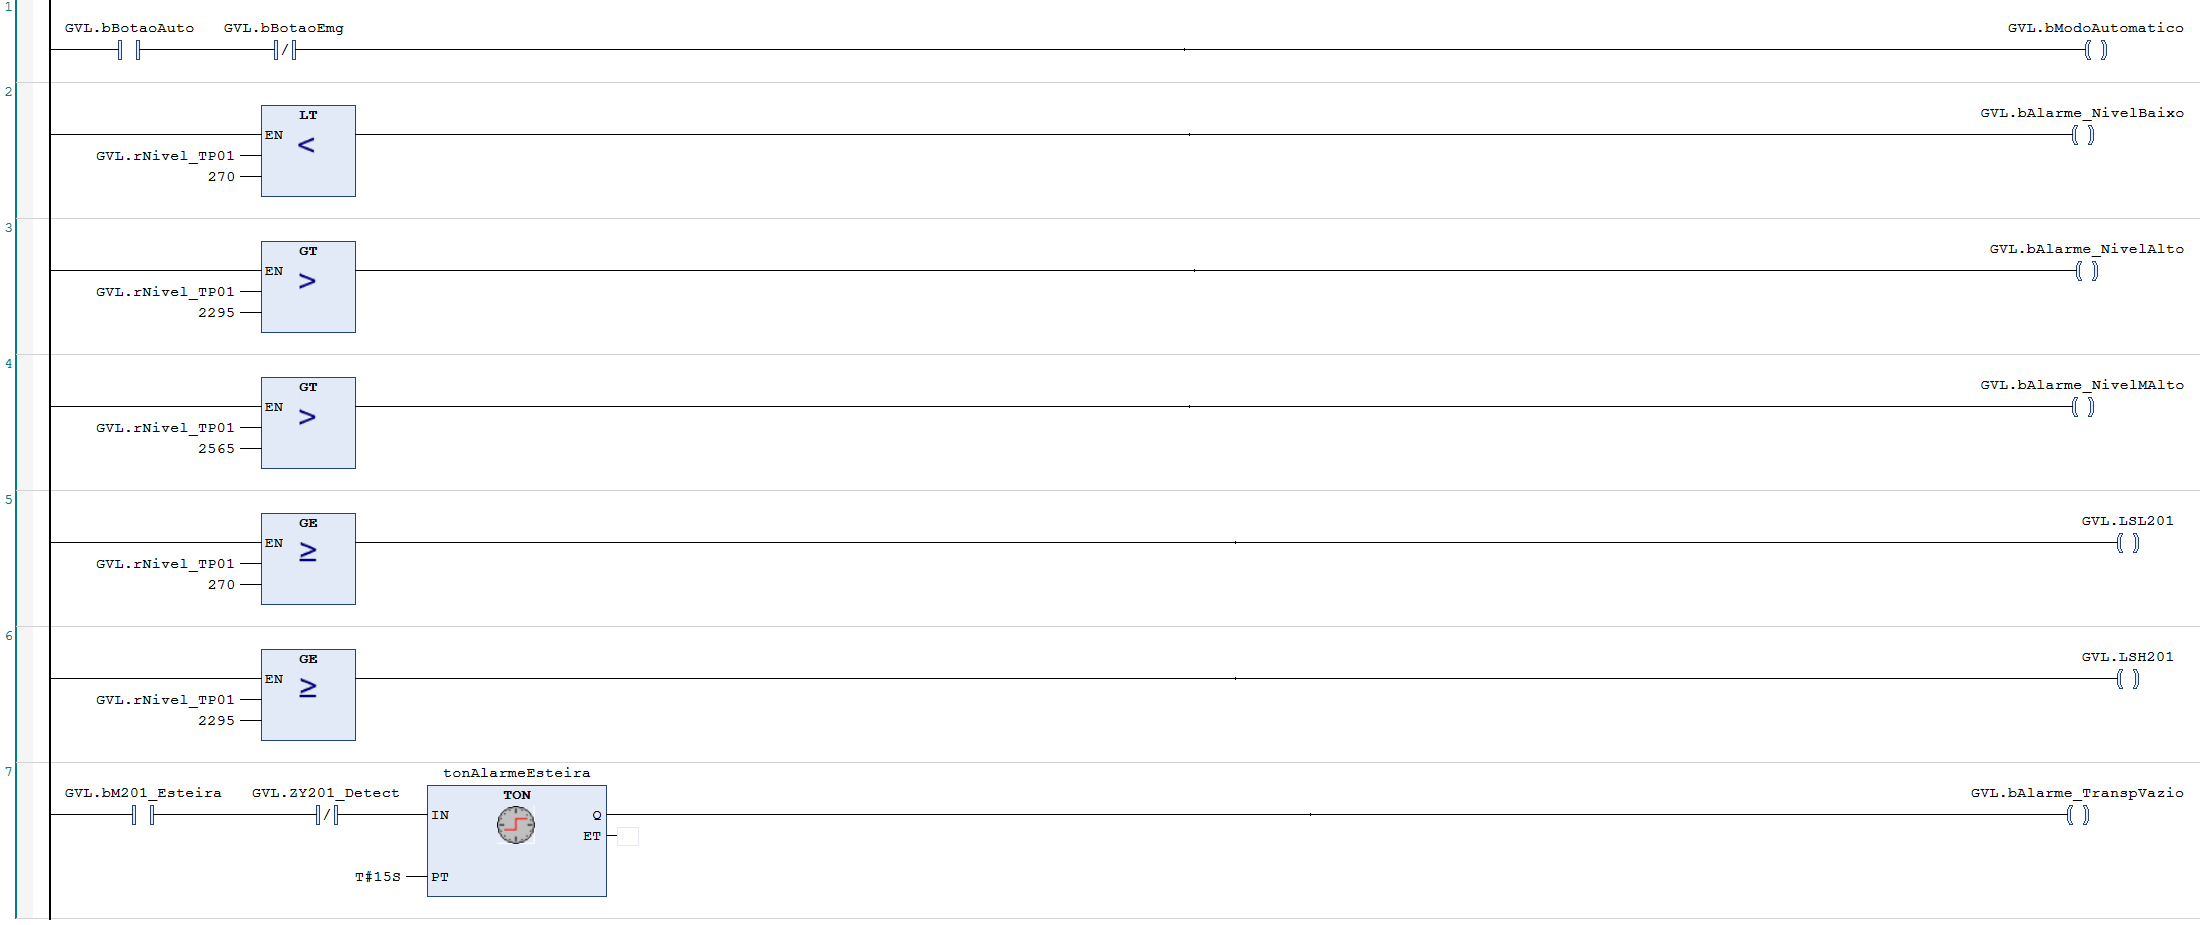
\includegraphics[width=1\textwidth]{imgs/Ladder-Prg.png}
    \caption{Lógica Ladder do controle de alarmes.}
\end{figure}

\subsection{Simulação dos Tanques (Prg\_Simulacao}

Este programa estrutura toda a lógica da planta, modelando desde o comportamento físico dos tanques até o controle automático das operações. Os blocos de tanques calculam nível, temperatura e estados das válvulas; os de dosagem controlam volumes de Gin e Vermouth com precisão; e o de mistura gerencia o motor via PWM com rampas de aceleração e resfriamento da jaqueta térmica. A transferência para o tanque pulmão é regulada por histerese de nível, enquanto a área de envase utiliza blocos para sincronizar sensores, esteira transportadora e a válvula de enchimento. Complementando o sistema, blocos de alarmes e segurança monitoram falhas (como ausência de barris), níveis críticos e condições de emergência, garantindo parada segura e intertravamentos adequados. Em conjunto, esses blocs modularizam o processo e permitem uma simulação realista e organizada conforme a IEC 61131-3.

\begin{figure}[H]\label{fig:ladder-simu}
    \centering
    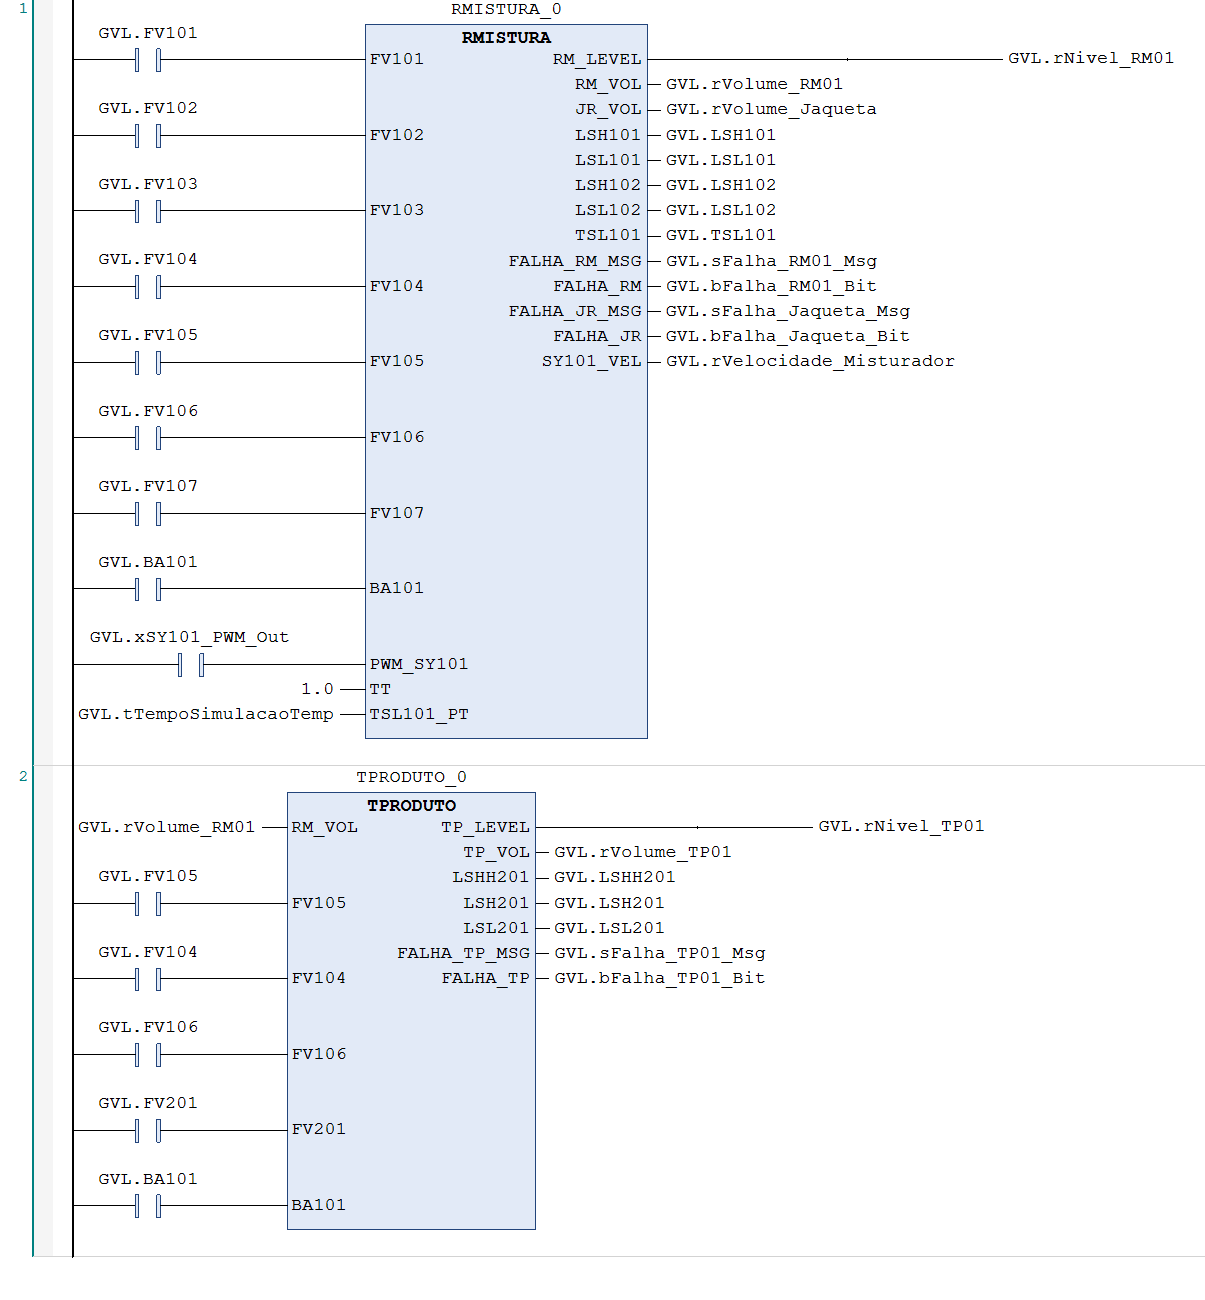
\includegraphics[width=1\textwidth]{imgs/Ladder_Simulacao.png}
    \caption{Lógica Ladder do controle dos Tanques.}
\end{figure}
\section{IHM}\label{sec:ihm}

A interface de operação e supervisão foi desenvolvida utilizando o software \textbf{InduSoft Web Studio}, estabelecendo comunicação com o controlador lógico através do driver \textbf{OPC UA} (Porta 4840). O desenvolvimento da tela seguiu os requisitos de animação e controle estipulados nas especificações do projeto.

\subsection{Sinótico Geral e Identidade Visual}
A tela principal apresenta um sinótico completo do processo, integrando as Áreas 01 (Batelada) e 02 (Envase). Para facilitar a interpretação rápida pelo operador, adotou-se a seguinte convenção visual para os atuadores (válvulas e motores):
\begin{itemize}
    \item \textbf{Cor Vermelha:} Indica que o equipamento está \textbf{Ativo/Ligado} ou a válvula está \textbf{Aberta}.
    \item \textbf{Cor Verde:} Indica que o equipamento está \textbf{Desligado} ou a válvula está \textbf{Fechada}.
\end{itemize}

\subsection{Detalhamento das Áreas}

\subsubsection{Reator de Mistura (RM-01)}
O tanque RM-01 possui animações dinâmicas que indicam o nível em tempo real, tanto por preenchimento gráfico vertical (\textit{Bar Graph}) quanto por display numérico em milímetros. O sinótico permite visualizar:
\begin{itemize}
    \item \textbf{Misturador:} O motor do misturador (\textbf{M-101}) altera sua cor quando ligado.
    \item \textbf{Resfriamento:} O estado da jaqueta de resfriamento é monitorado, indicando o estado normal (cinza) ou resfriado (azul claro).
    \item \textbf{Sensores:} O status dos sensores de nível (LSH-101, LSH-102, LSL-101, LSL-102) e temperatura (TSL-101) é indicado por "LEDs" virtuais que alteram de cor conforme a atuação.
\end{itemize}

\subsubsection{Tanque de Produto (TP-01) e Transferência}
O tanque de armazenamento (TP-01) exibe o nível acumulado do produto Dry Martini pronto para o envase. A interface monitora as chaves de nível (LSHH-201, LSH-201, LSL-201) e controla a bomba de transferência \textbf{BA-101}, permitindo ao operador acompanhar o esvaziamento do reator e o enchimento dos barris.

\subsubsection{Sistema de Envase e Transporte (TR-01)}
A esteira transportadora foi animada para representar o fluxo contínuo de produção. Os principais elementos visuais incluem:
\begin{itemize}
    \item \textbf{Movimentação:} Animação dos barris deslocando-se sobre a esteira quando o motor \textbf{M-201} está ativo.
    \item \textbf{Sensores de Proximidade:} Os sensores \textbf{ZY-201} (posicionamento para envase) e \textbf{ZY-202} (contagem de saída) indicam visualmente a detecção dos barris.
    \item \textbf{Bico Injetor:} Animação da válvula \textbf{FV-201} e do fluxo de líquido, que só ocorre quando um barril é validado pelo sensor de posicionamento.
    \item \textbf{Contador de barris:} Indica visualmente a contagem dos barris.
\end{itemize}

\subsection{Modos de Operação e Intertravamentos}

A seleção do modo de operação é realizada através de botões dedicados no painel de comando da IHM, alternando o comportamento do sistema entre \textbf{Automático (AUTO)} e \textbf{Manual (MAN)}:

\begin{itemize}
    \item \textbf{Modo Automático:} Ao ser ativado, o controlador assume a execução lógica da batelada e do envase sequencial. Neste estado, os botões de acionamento individual dos equipamentos (válvulas e motores) são bloqueados na interface, impedindo interferência humana indevida durante a produção.
    
    \item \textbf{Modo Manual:} Ao selecionar este modo, a lógica de sequenciamento é interrompida, e o operador ganha permissão para atuar individualmente sobre cada componente. Na IHM, isso libera o comando de todas as válvulas (FV-101 a FV-107, FV-201), do motor do misturador (M-101), da bomba (BA-101) e do motor do transportador (M-201).
\end{itemize}

Visualmente, a IHM indica o modo ativo, garantindo que o operador esteja sempre ciente do estado de controle da planta.

\subsection{Gerenciamento de Dados e Alarmes}
No canto superior esquerdo, um painel de \textbf{Totalização} exibe os volumes de Gin e Vermouth da batelada atual e os volumes acumulados de Gin, Vermouth e Produto Final ao longo de toda a produção, além de um contador específico para o número de bateladas realizadas.

O sistema conta ainda com:
\begin{itemize}
    \item \textbf{Objeto de Alarmes:} Localizado na parte inferior ("Mensagens"), registra e exibe as falhas e eventos do sistema, ou seja, indica quando o nível do TP-01 está baixo, alto ou muito alto, além de mostrar quando o transportador ficar vazio por mais tempo do que deveria. É possível o operador silenciar ou reconhecer os alarmes dando dois cliques na mensagem.
    \item \textbf{Botão de Emergência:} Disponível em destaque na tela, possui lógica retentiva. Visualmente, o botão indica o estado \textit{True} (acionado/seguro) através da cor \textbf{Verde}, indicando a parada imediata do processo em situações críticas.
\end{itemize}

%  PRINT DA IHM AQUI
\begin{figure}[H]
    \centering
    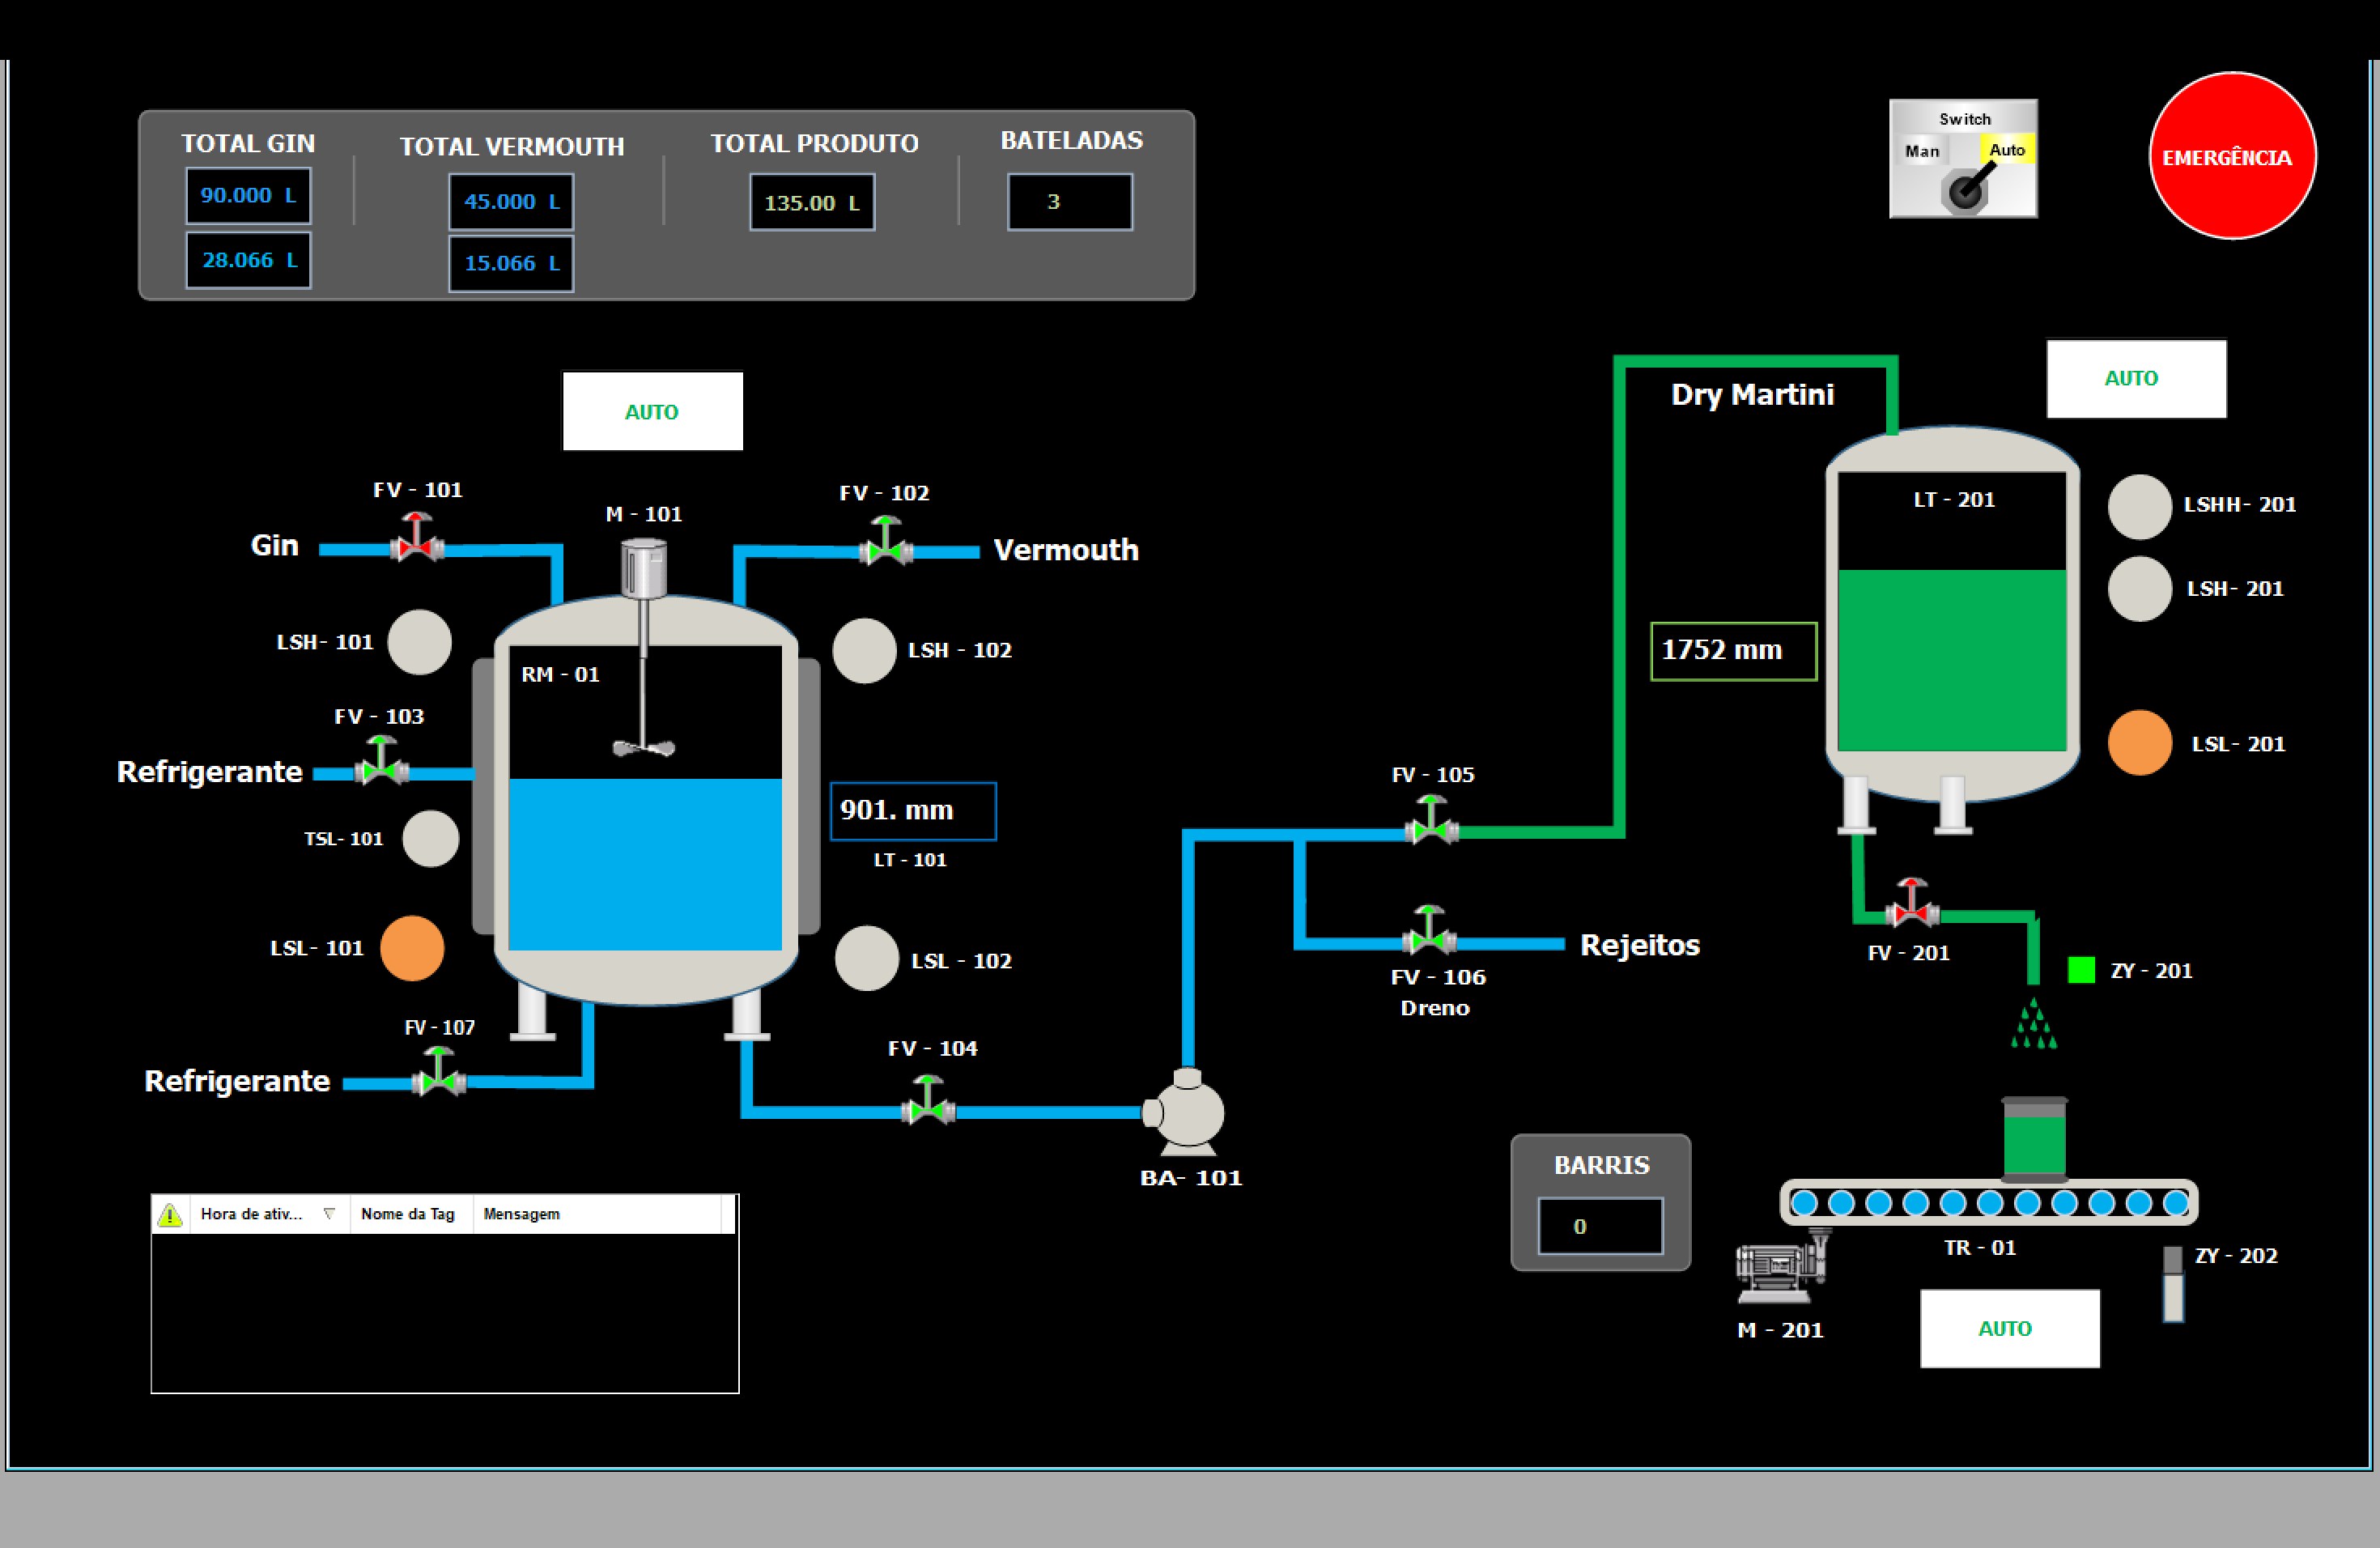
\includegraphics[width=0.8\textwidth]{imgs/print_ihm.png}
    \caption{Tela Principal do Supervisório em funcionamento.}
\end{figure}
\section{Testes Realizados}\label{sec:testes}

O sistema foi validado através de simulação conectada (CODESYS + InduSoft).

\subsection{Teste de Controle PWM do Misturador}
Validou-se a rampa de aceleração e desaceleração do motor M-101 (Misturador). Através da ferramenta \textit{Trace} do CODESYS, constatou-se que o sinal PWM atingiu 100\% do ciclo de trabalho em 5 segundos na partida, e retornou a 0\% em 10 segundos na parada, cumprindo o requisito de partida suave especificado.

\begin{figure}[H]
    \centering
    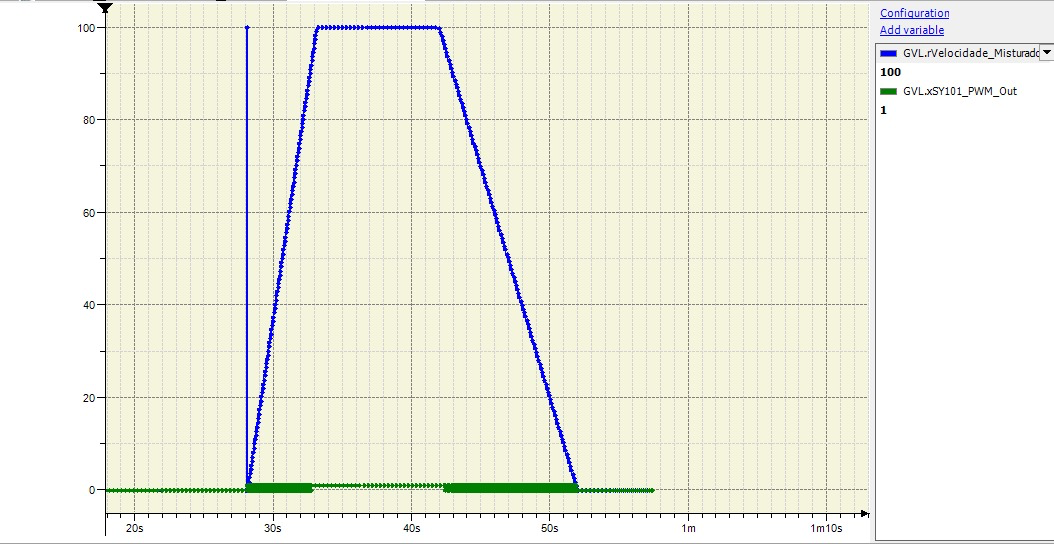
\includegraphics[width=0.6\textwidth]{imgs/pwm.png}
    \caption{Gráfico do PWM.}
\end{figure}

\subsection{Teste Área 1: Tanque RM-01}
Verificou-se o enchimento do tanque RM-01 a partir da atuação das válvulas de Gin e Vermouth, além do display de seu nível ao lado. Após as devidas proporções adicionadas, o misturador M-101 foi acionado. O ciclo de resfriamento da jaqueta foi verificado simulando os sensores de nível e temperatura. A válvula de refrigerante (FV-103) abriu corretamente ao iniciar a mistura e fechou imediatamente ao acionar o sensor de nível alto da jaqueta (LSH-102). 

\begin{figure}[H]
    \centering
    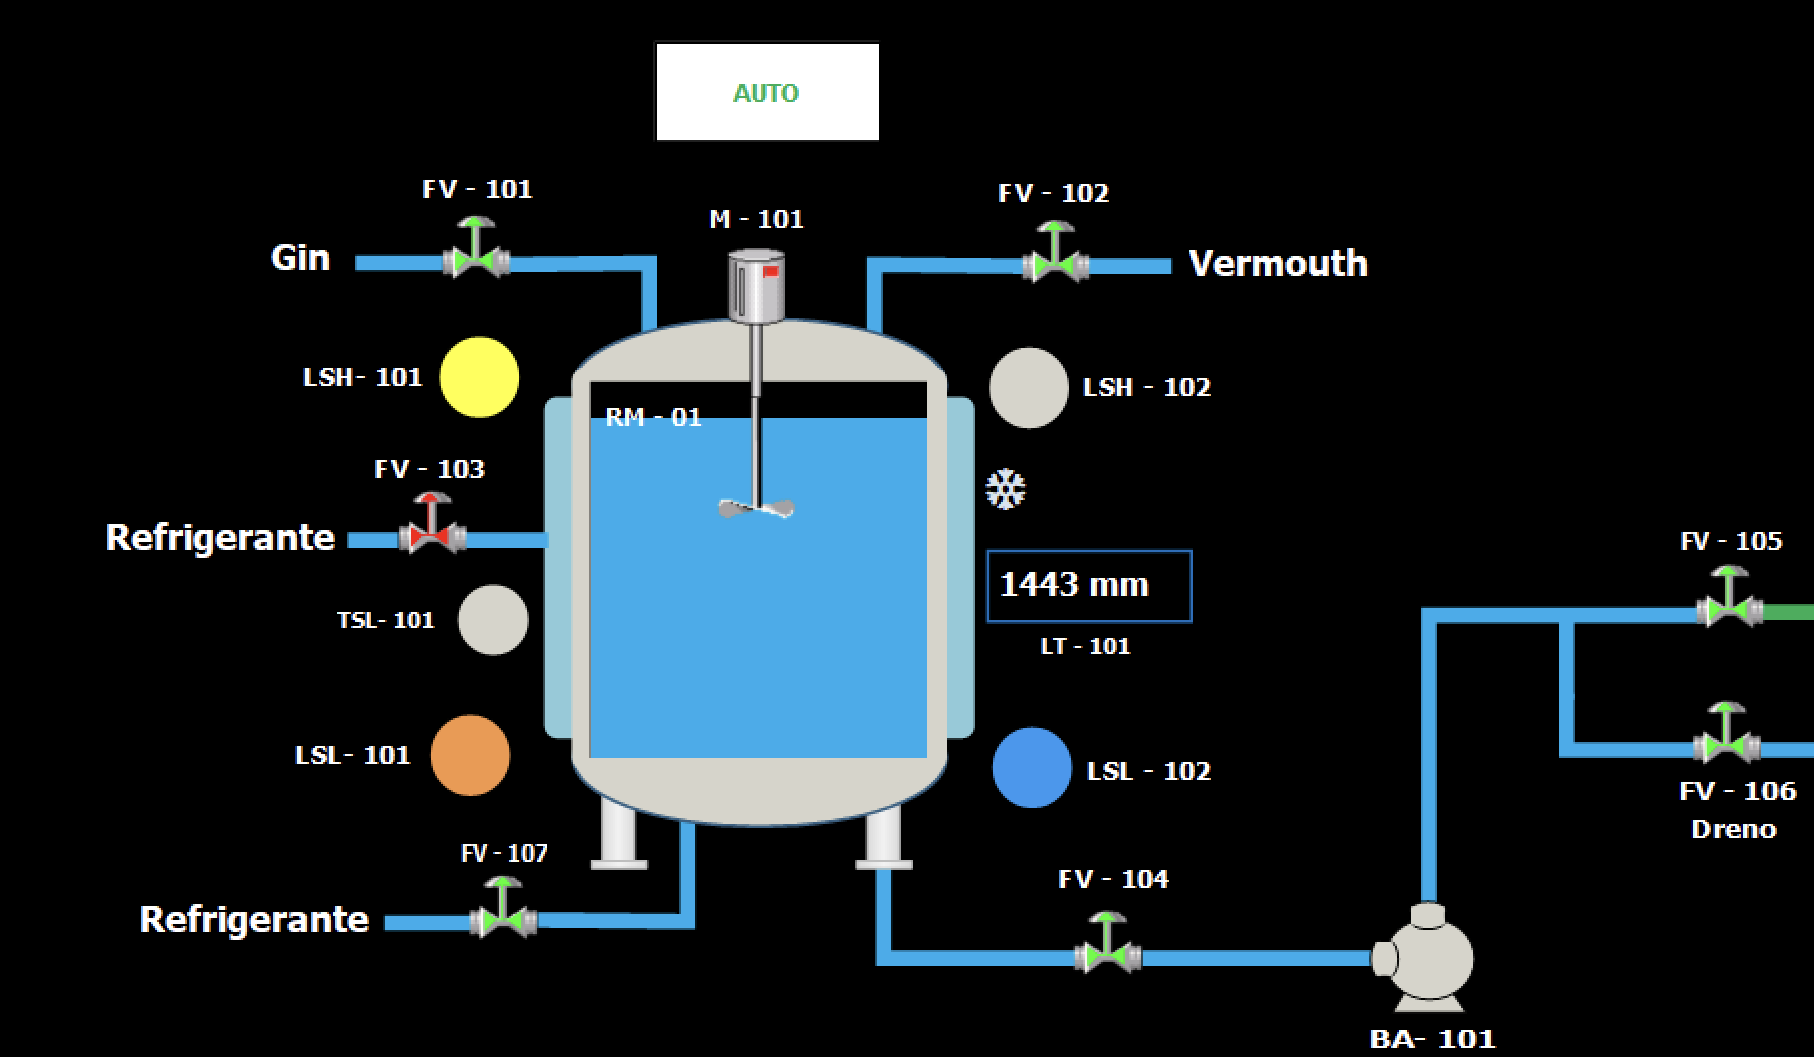
\includegraphics[width=0.6\textwidth]{imgs/rm_01.png}
    \caption{Tanque RM-01 com o misturador e a jaqueta em funcionamento.}
\end{figure}

\subsection{Teste de Envase}
Validou-se o funcionamento da Área 2: o TP-01 recebe o produto após a atuação das válvulas e da bomba BA-101 e, a partir da atuação da esteira, começa a encher os barris. A esteira só entra em operação quando o nível do Tanque de Produto supera 50\%, e desliga automaticamente quando o nível cai abaixo de 10\%, evitando oscilação do motor. Tudo isso com a correta implementação do sensor ZY-201, que identifica a presença do barril, e com a animação devida do bico injetor. Após o enchimento do barril, ele vai para o final da esteira, onde o sensor ZY-202 faz a contagem.

\begin{figure}[H]
    \centering
    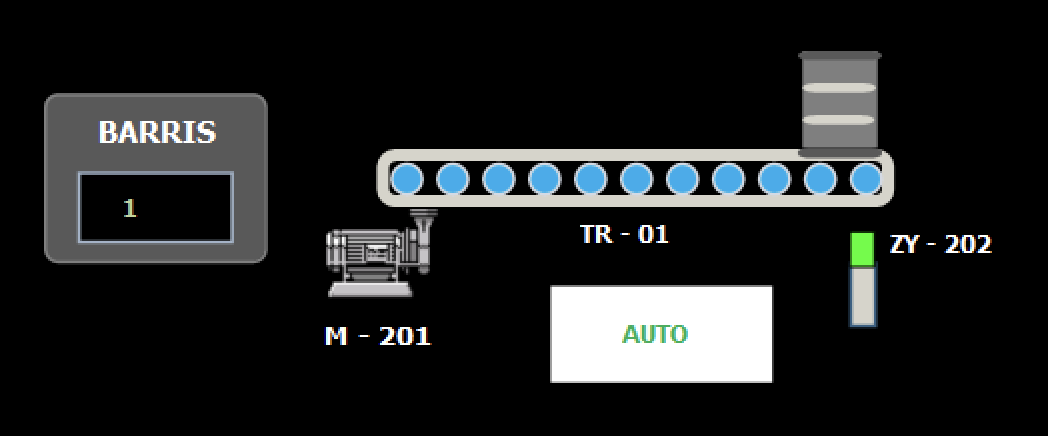
\includegraphics[width=0.6\textwidth]{imgs/contagem_barril.png}
    \caption{Contagem dos barris.}
\end{figure}

\subsection{Teste de Emergência}
Ao acionar o botão de Emergência durante a fase de mistura, o sistema interrompeu imediatamente o motor e as válvulas. Após o tempo de segurança (3s), a rota de descarte para o Tanque de Rejeitos foi aberta, validando a lógica de segurança implementada no SFC.
\begin{figure}[H]
    \centering
    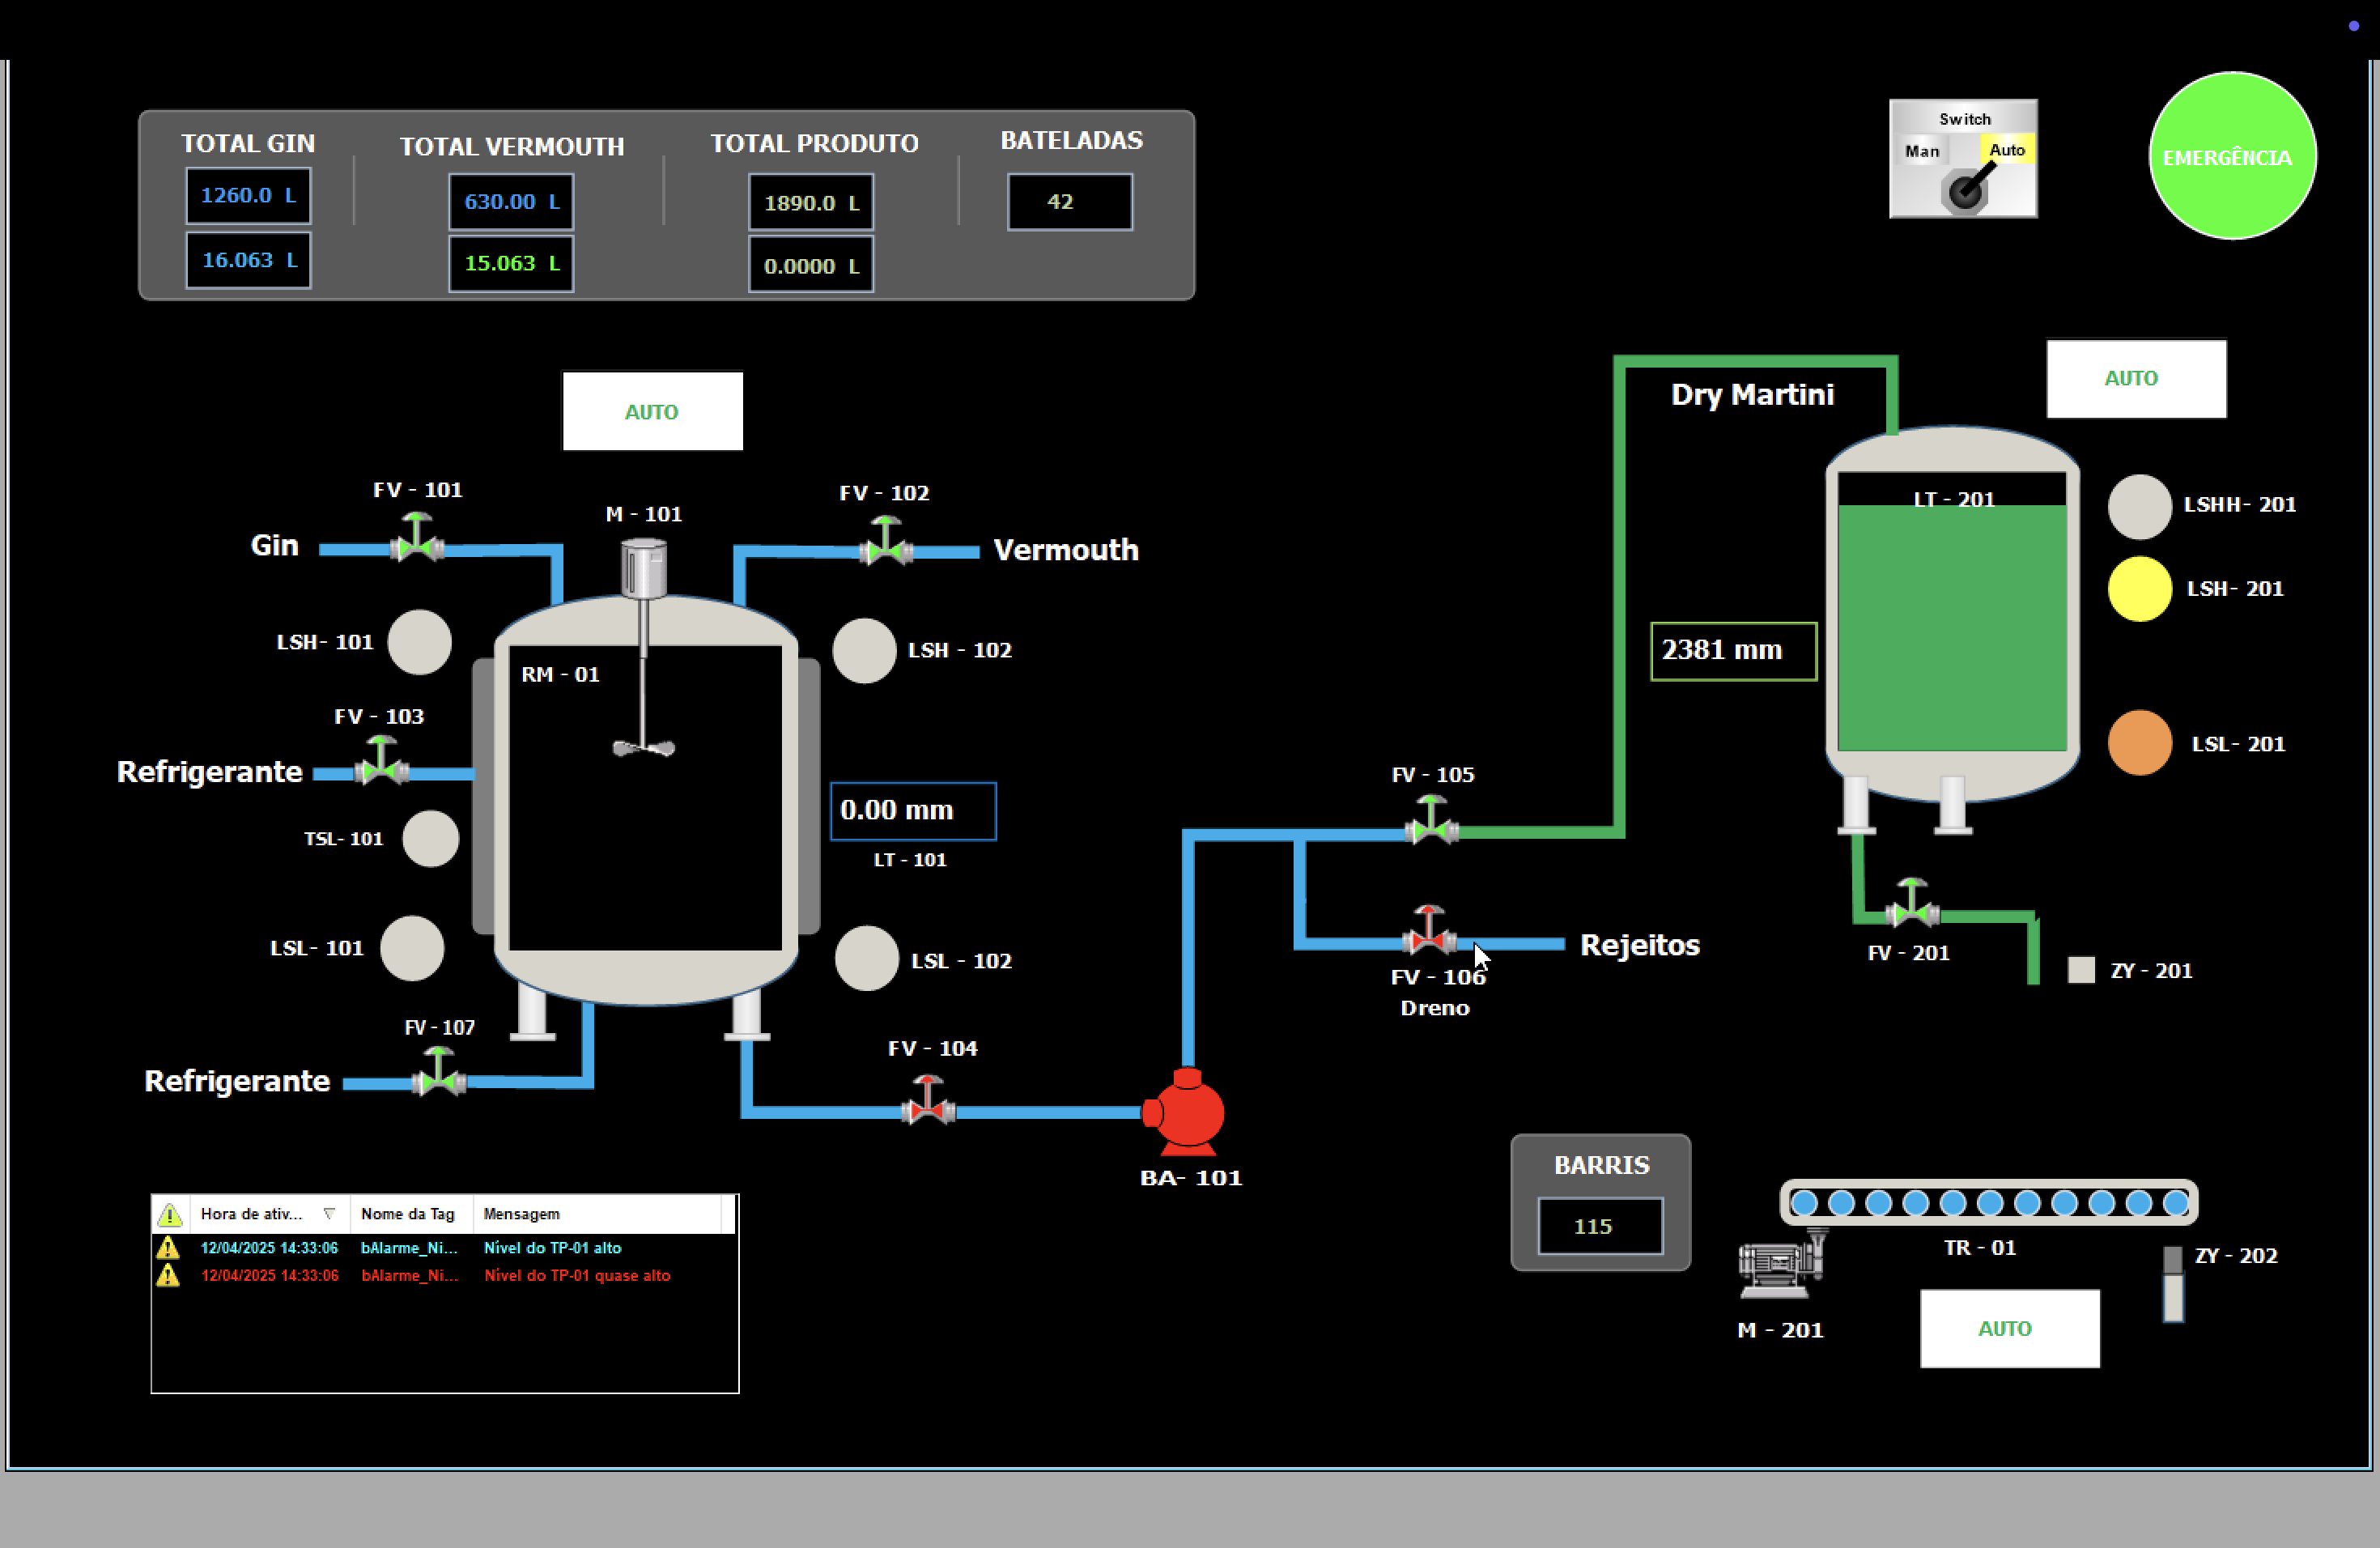
\includegraphics[width=0.6\textwidth]{imgs/emg_funcionando.png}
    \caption{Drenagem após apertar o botão de emergência.}
\end{figure}

\subsection{Validação dos Modos de Operação}
Alternou-se o sistema para o modo MANUAL na IHM. Verificou-se que a lógica sequencial (SFC) foi congelada e que o operador obteve controle individual sobre cada atuador (válvulas, bomba e motores), permitindo manobras de manutenção sem restrições de intertravamento lógico. Cada setor da tela do sinótico possui um identificador de qual modo está operando.

\subsection{Sensores, Totalizadores e Alarmes}
Todos os sensores discretos funcionam corretamente, identificando os respectivos níveis de seus tanques. Além disso, os totalizadores fazem a contagem correta da quantidade de cada produto, ciclo e barril, sendo mostrados em displays. Por fim, os alarmes mostram as mensagens correspondentes, podendo ser silenciados ou reconhecidos. 

\begin{figure}[H]
    \centering
    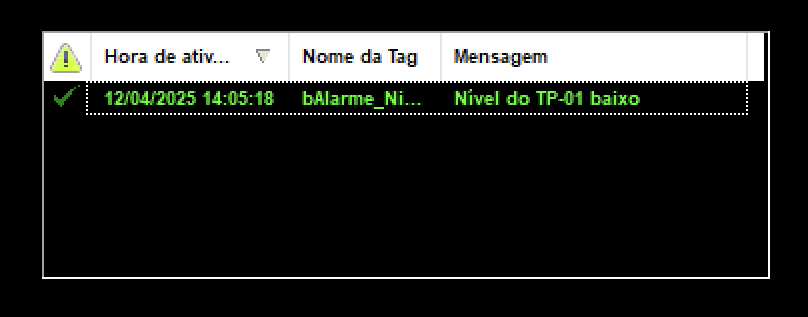
\includegraphics[width=0.5\textwidth]{imgs/reconhecimento_alarme.png}
    \caption{Reconhecimento de um alarme.}
\end{figure}

\begin{figure}[H]
    \centering
    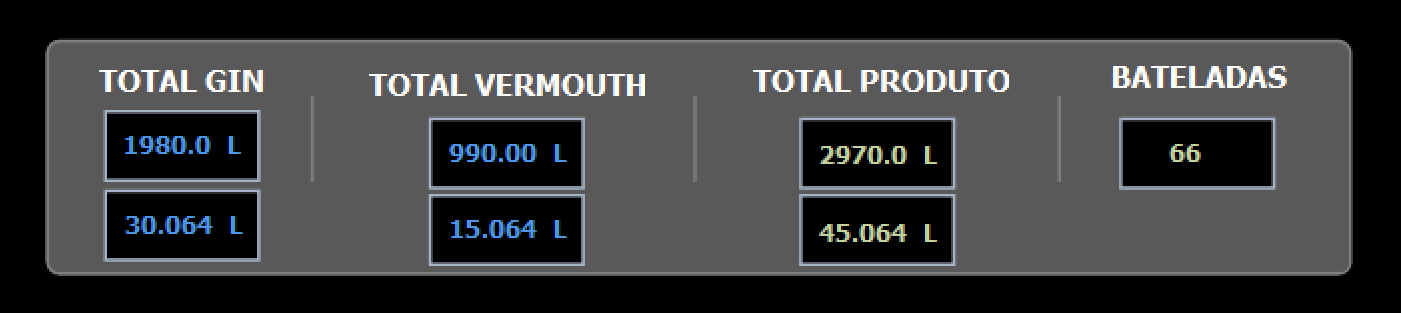
\includegraphics[width=0.5\textwidth]{imgs/totalizadores.png}
    \caption{Totalizadores mostrando a quantidade dos produtos e bateladas.}
\end{figure}

\section{Conclusão}\label{sec:conclusao}

O projeto permitiu a implementação prática dos conceitos de automação industrial seguindo a norma IEC 61131-3. A arquitetura multitarefa mostrou-se essencial para simular a física do processo sem comprometer o tempo de varredura da lógica de controle. A integração via OPC UA com o supervisório proporcionou uma operação robusta e visual, atendendo a todos os requisitos funcionais propostos, incluindo modos de operação, alarmes e rotinas de segurança.


%%%%%%%%%%%%%%%%%%%%%%%%%%%%%%%%%%%%%%%%%%%%%%%%%%%%%
%%%%%%%%%%%%%%%%%%%%%%%%%%%%%%%%%%%%%%%%%%%%%%%%%%%%%


%bibliografia
\bibliographystyle{unsrt}
\bibliography{resources/bibliografia}

\end{document}